\documentclass[12pt,a4paper,titlepage,oneside]{report}

%%{{{ packages
%% font encoding.
\usepackage[utf8]{inputenc}
\usepackage[T1]{fontenc}
\usepackage{lmodern}
\usepackage{couriers}
%% Customize chapters.
\usepackage{titlesec}
%% bibliography.
\usepackage[backend=bibtex,style=ieee]{biblatex}
%% \includegraphics{name}
\usepackage{graphicx}
%% \url{something}
\usepackage{url}
%% \multirow{package}{width}{text}
\usepackage{multirow}
%% \cellcolor
\usepackage[table]{xcolor}
%% \caption{title}
\usepackage{caption}
\usepackage{subcaption}
%% \forloop
\usepackage{forloop}
%% fix underfull on footnote with URL.
\usepackage{ragged2e}
%% source code listing
\usepackage{listings}
%% \printindex
\usepackage{makeidx}
%% table of content
\usepackage{tocloft}
%% text emphasis, including strikeout.
\usepackage[normalem]{ulem}
%% mathematics
\usepackage{mathtools}
%% arithmetic
\usepackage{calc}
%% algorithm
\usepackage{algorithm}
\usepackage{algpseudocode}
%% multiple columns
\usepackage{multicol}
%% Change the margin
\usepackage[a4paper]{geometry}
\geometry{
	a4paper,
	top=3cm,
	right=3cm,
	bottom=3cm,
	left=4cm
}
%%
\usepackage{parskip}
%% Package for reading CSV to database.
\usepackage{datatool}
%% Package for scatter and line plot.
\usepackage{dataplot}
%% Long table
\usepackage{longtable}
%% Tikz
\usepackage{pgfplots}

%% Add box to figure.
%%
\usepackage{float}

\floatstyle{boxed}
\restylefloat{figure}

%% MnSymbol
\usepackage{MnSymbol}
%%}}}

%%{{{ hyphenation: sorted in ascending.
%%
\hyphenation{
	Ja-nu-a-ri
	SIGKDD
	Wiki-pedia
	a-kan
	ang-ka
	ba-gai-ma-na
	bayes-ian
	ber-kas
	ber-ma-sa-lah
	ber-mak-na
	bi-a-ya
	da-lam
	data-set
	de-ngan
	di-ha-sil-kan
	di-sing-kat
	di-tam-bah-kan
	dis-krit
	fung-si
	ga-bung-an
	ke-las
	ke-mung-ki-nan
	ke-tak-se-imbang-an
	lan-guage
	ma-yo-ri-tas
	me-laku-kan
	me-me-rik-sa
	me-mi-lih
	me-ne-rap-kan
	me-ning-kat-kan
	me-nye-dia-kan
	me-nye-im-bang-kan
	me-sin
	me-thod
	mem-vi-sua-li-sa-si
	meng-gu-na-kan
	meng-hu-bung-kan
	meng-i-kut-kan
	meng-i-kuti
	meng-im-ple-men-ta-si-kan
	meng-in-di-ka-si-kan
	mi-sal-nya
	mung-kin
	o-ver-sam-pling
	pa-ra-lel
	pe-mi-sah
	pe-nan-da
	pe-ne-li-ti-an
	pe-nu-li-san
	pe-nyun-ting
	pem-ban-ding
	pen-de-kat-an
	peng-kla-si-fi-ka-si
	per-for-man-si-nya
	po-ten-si-al
	pro-ba-bi-li-tas
	pro-ses
	sam-pel
	se-im-bang
	se-jum-lah
	sun-ting-an
	ting-kat
	un-der-sam-pling
	wa-lau-pun
}
%%}}}

%%{{{ override default latex setting.
%%

%% Space between paragraphs.
\setlength{\parskip}{1.5em}

%% Add dot to TOC.
\renewcommand{\cftsecleader}{\cftdotfill{\cftdotsep}}
\renewcommand{\contentsname}{}

\lstset{
	basicstyle=\scriptsize\ttfamily
,	breaklines=true
,	stringstyle=\scriptsize\ttfamily
,	numbers=left
,	numberstyle=\tiny\ttfamily
,	numbersep=5pt
,	tabsize=4
,	frame=single
}

\makeatletter
\def\lst@lettertrue{\let\lst@ifletter\iffalse}
\makeatother

%% Format chapter and section.
%%
%%% Set chapter name to Bab.
\titleformat{\chapter}[hang]
{\bfseries\large\centering}
{Bab \thechapter}
{1em}
{}

\titleformat{\section}[hang]
{\bfseries\large}
{\thesection}
{1em}{}

%% Set spacing for sections.
\titlespacing{\chapter}{0ex}{0ex}{1.5em}
\titlespacing{\section}{0ex}{0ex}{0em}

%% Alter latex default title on table.
\captionsetup[table]{name=Tabel}
\captionsetup[figure]{name=Gambar}

\renewcommand{\arraystretch}{1.5}
\setlength{\tabcolsep}{3pt}

%% Change bibliography title.
\defbibheading{bibliography}{\centerline{
	\textbf{DAFTAR REFERENSI}}
}

%%% uncomment this to show overrule in black box
\overfullrule=2cm

%% Algorithmicx
\makeatletter
\renewcommand{\ALG@beginalgorithmic}{\footnotesize}
\makeatother

%% multicolumn setting
\setlength{\columnsep}{1cm}

%% pgfplots setting.
\pgfplotsset{
	/pgf/number format/read comma as period,
	/pgf/text mark as node=false,
	table/col sep=semicolon,
	xmax=1,
	xmin=0,
	ymax=1,
	ymin=0,
	xtick distance=0.2,
	ytick distance=0.2,
	grid=major,
	cycle list name=linestyles,
}
%%}}}

%%{{{ variables
%%
\newcommand{\mytitle}{Deteksi Vandalisme pada Wikipedia Bahasa Inggris menggunakan klasifikasi Cascaded Random Forest}
\newcommand{\myname}{Muhamad Sulhan}
\newcommand{\mysid}{23513014}
\newcommand{\myadvisorname}{Dwi Hendratmo Widyantoro}
\newcommand{\myadvisorid}{196812071994021001}
\newcommand{\mydept}{Program Studi Magister Informatika}
\newcommand{\itb}{Institut Teknologi Bandung}

%%% My images directory
\graphicspath{{../images/}}
\newcommand{\myitbcover}{ITB-logo-hitam}

%%% My bibligraphy file
\addbibresource{bibliography.bib}
%%}}}

%%{{{ document's meta-data
%%
\author{\myname}
\title{\mytitle}
%%}}}

%%{{{ document's macros
%%
%%% two column signature.
\def\myadvisorsig#1{%
	\vbox{\hsize=6cm
		\textbf{#1}\\
		\addvspace{2cm}%
		\hbox to \hsize{%
			\strut\hfil%
			\myadvisorname%
			\hfil%
		}
		\hrule\kern1ex
		\hbox to \hsize{%
			\strut\hfil%
			NIP\hspace{1ex}\myadvisorid%
			\hfil%
		}
	}
}

%%% one column signature.
\def\mysignature#1#2#3{%
	\vbox{
		\textbf{#1}\\
		\addvspace{2cm}%
		\hbox to \hsize{%
			\strut\hfil%
			{#2}%
			\hfil%
		}
		\makebox[6cm][c]{
			\hrulefill
		}
		\hbox to \hsize{%
			\strut\hfil%
			NIP\hspace{1ex}{#3}%
			\hfil%
		}
	}
}

%%% source code listing
\lstdefinelanguage{go}
{
	morekeywords={package,import,const,func,for,type,var,struct}
,	sensitive=true
,	morecomment=[l]{//}
,	morecomment=[s]{/*}{*/}
}
\lstdefinestyle{go}{%
	language=go
,	keywordstyle=\color{black}\bfseries
,	commentstyle=\color{gray}
,	breakatwhitespace=true
,	lineskip={-2.5pt}
}
\newcommand{\includecodego}[2][c]{
	\lstinputlisting[caption=#2,escapechar=,style=go]
		{/home/ms/go/work/src/github.com/shuLhan/#2}
}

%%% data listing
\lstdefinestyle{data}{%
	breakatwhitespace=false
,	breakautoindent=false
,	literate={\,}{}{0\discretionary{,}{}{,}},
}
\newcommand{\includedata}[2][c]{
	\lstinputlisting[caption=#2,style=data,linerange={1-10}]
		{/home/ms/go/work/src/github.com/shuLhan/#2}
}
%%}}}

%%
%% Create cover with parameters
%% 1: report number
%% 2: report weeks, in string
%% 3: report date, string
%%
\newcommand{\reportcover}[3]{
	\thispagestyle{empty}
	\begin{center}\textbf{%
		\mytitle
		\vfill
		Laporan Progres Tesis, Catatan, dan Pekerjaan Selanjutnya
		\linebreak
		Laporan ke-#1
		\linebreak
		Minggu #2
		\linebreak
		\linebreak
		#3
		\vfill
		Oleh \\
		\myname \\
		\mysid \\
		\vfill
		\uppercase{%
			Program Studi Magister Informatika \\
			Sekolah Teknik Elektro dan Informatika \\
			Institut Teknologi Bandung \\
			2015
		}
	}
	\end{center}
	\newpage
}

%%
%% Macro for advisor's signature
%%
\newcommand{\advisorsignature}{
	\vfill
	\begin{center}
		Diketahui oleh,
		\linebreak
		\linebreak
		\hbox to \hsize{%
			\myadvisorsig{Pembimbing,\quad}\hfil
		}
	\end{center}
}

%%
%% Macro for create schedule using parameter
%% 1: number of weeks has passed on task 1
%% 2: number of weeks has passed on task 2
%% 3: number of weeks has passed on task 3
%% 4: number of weeks has passed on task 4
%% 5: should we begin in newpage?
%%

% function to fill cell with color
\newcommand{\tand}{&}
\newcounter{cnt}
\newcommand{\fillcell}[1]{%
	\forloop{cnt}{0}{\value{cnt}<#1}{%
		{\cellcolor[gray]{0.7}} \tand
	}%
}
% function to create empty cell
\newcommand{\emptycell}[2]{%
	\forloop{cnt}{0}{\value{cnt}<#1}{%
		\tand
	}%
	\ifthenelse{#2 = 1}{\\}{\tand}%
}
% function to fill week in progress.
\newcommand{\progresscell}[1]{%
	\forloop{cnt}{0}{\value{cnt}<#1}{%
		{\cellcolor{red!80}} \tand
	}%
}

\newcommand{\schedule}[4]{
	\section{Penjadwalan}\label{sec:penjadwalan}

Tabel di bawah menampilkan jadwal yang direncanakan dalam pengembangan tesis dari bulan ke I, September 2015, sampai dengan bulan ke VI, Januari 2016.

Warna merah menandakan minggu yang telah lewat sampai minggu dari laporan progres ini, untuk warna abu-abu menandakan waktu pelaksanaan yang akan datang.

\newcounter{planone}
\newcounter{plantwo}
\newcounter{planthree}
\newcounter{planfour}

\newcounter{progressone}
\newcounter{progresstwo}
\newcounter{progressthree}
\newcounter{progressfour}

\setcounter{progressone}{#1}
\setcounter{progresstwo}{#2}
\setcounter{progressthree}{#3}
\setcounter{progressfour}{#4}

\setcounter{planone}{4 - \theprogressone}
\setcounter{plantwo}{17 - \theprogresstwo}
\setcounter{planthree}{14 - \theprogressthree}
\setcounter{planfour}{2 - \theprogressfour}

\begin{table}[h!]
	\centering
	{\footnotesize
	\begin{tabular}{|c|p{0.2\textwidth}
	|c|c|c|c
	|c|c|c|c
	|c|c|c|c
	|c|c|c|c
	|c|c|c|c
	|c|c|c|c|}
		\hline
		\multirow{2}{*}{No.}
			& \multirow{2}{*}{Kegiatan}
			& \multicolumn{4}{c|}{Bulan I}
			& \multicolumn{4}{c|}{Bulan II}
			& \multicolumn{4}{c|}{Bulan III}
			& \multicolumn{4}{c|}{Bulan IV}
			& \multicolumn{4}{c|}{Bulan V}
			& \multicolumn{4}{c|}{Bulan VI}\\
		\cline{3-26}
		& &
			1 & 2 & 3 & 4 &
			1 & 2 & 3 & 4 &
			1 & 2 & 3 & 4 &
			1 & 2 & 3 & 4 &
			1 & 2 & 3 & 4 &
			1 & 2 & 3 & 4\\
		\hline
		1 & Persiapan\ \  Data dan\ \ Lingkungan Penelitian &
			\progresscell{\theprogressone}
			\fillcell{\theplanone}
			\emptycell{19}{1}
		\hline
		2 & Implementasi dan Pengujian &
			\emptycell{2}{0}
			\progresscell{\theprogresstwo}
			\fillcell{\theplantwo}
			\emptycell{3}{1}
		\hline
		4 & Analisis &
			\emptycell{7}{0}
			\progresscell{\theprogressthree}
			\fillcell{\theplanthree}
			\emptycell{1}{1}
		\hline
		5 & Evaluasi &
			\emptycell{20}{0}
			\progresscell{\theprogressfour}
			\fillcell{\theplanfour}
			\emptycell{0}{1}
		\hline
	\end{tabular}
	}
	\caption{Jadwal penelitian tesis}
\end{table}
}




\begin{document}
\reportcover{V}{17}{12 Januari 2016}

\section{Pendahuluan}

\subsection{Perbaikan Algoritma CART}

Kesalahan yang dilakukan pada implementasi sebelumnya yaitu pada penggunaan
atribut untuk pemisahan \textit{tree}.
Jika sebuah atribut telah digunakan sebagai pemisah, dan menjadi sebuah
\textit{node} pada pohon keputusan, maka atribut tersebut tidak boleh diproses
atau menjadi pemisah kembali pada anak-anaknya, namun bisa diproses kembali
pada \textit{grandchild}-nya.

Hal seperti ini tidak pernah disebutkan dalam teks algoritma CART,
sehingga saya cukup kesulitan menemukan kesalahan yang dilakukan.

\subsection{Implementasi Random Forest}

Implemetansi algoritma \textit{ensemble} \textit{Random Forest} (RF) secara
umum mengacu pada buku Friedman, dkk. \cite{friedman2001elements}, dengan
tambahan dari video kuliah dan tulisan lain di internet.

Algoritma RF yang diimplementasikan menggunakan teknik \textit{bagging},
\textit{out-of-bag} (OOB), dan CART sebagai pengklasifikasi di setiap pohon
keputusan.

\clearpage

Berikut algoritma RF yang digunakan,

\begin{lstlisting}
FUNGSI RandomForest
INPUT
	D: dataset
	NTREE: jumlah tree
	NFEATURE: jumlah fitur yang dipilih secara acak
	NBAGGING: jumlah sub-sampel yang dipilih secara acak dengan
	replacement, dalam nilai persentase.
OUTPUT
	FOREST: kumpulan tree
VAR
	SUMOOBERROR: total galat untuk OOB
BEGIN
	SUMOOBERROR := 0.0

	FOR i = 0; i < NTREE; i++
	BEGIN
		subsample, oob := RandomPickRows(D, NBAGGING)

		subfeature := RandomPickColumns(subsample, NFEATURE)

		cartTree := CreateTree(subfeature)

		ooberror := cartTree.CountOOBError(oob)

		SUMOOBERROR += ooberror

		FOREST.AddTree(cartTree)
	END

	FOREST.AverageOOBError = SUMOOBERROR / NTREE
END
\end{lstlisting}

Hasil implementasi kemudian diuji dengan dataset \textit{Glass Identification}
\cite{evett1987rule}, dengan jumlah sample yaitu 124, jumlah fitur 9, jumlah
kelas yaitu 7 (contoh data bisa dilihat pada lampiran
\ref{appendix:dataset_glass}),
Hasilnya dalam bentuk grafik penghitungan laju galat OOB yang dapat dilihat
pada gambar \ref{fig:rf_glass}.

\begin{figure}[t]
	\centering
	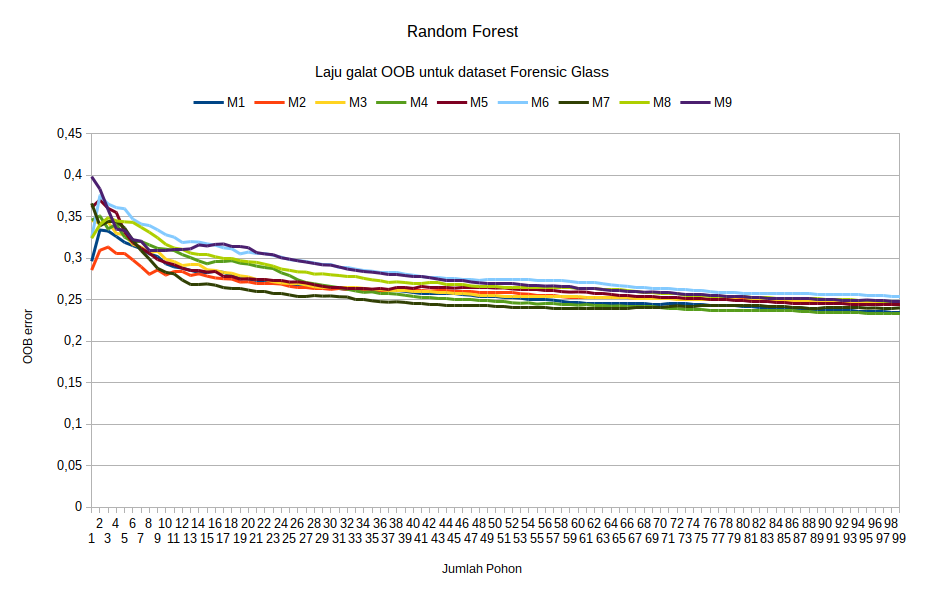
\includegraphics[keepaspectratio=true,scale=0.5]{rf_glass}
	\caption{OOB laju error pada Random Forest untuk dataset Forensic Glass
	dengan jumlah fitur secara acak dari 2 sampai 9.}
	\label{fig:rf_glass}
\end{figure}

Dataset diuji dengan mengambil dua per tiga (66\%) dari data asli untuk
\textit{bootstrap} dan sisanya digunakan sebagai latihan (OOB) untuk
mendapatkan galat, dengan jumlah tree yang digunakan yaitu 50.

\begin{itemize}
\item \textbf{Minggu 15, 16}. Perbaikan program CART dan implementasi Random
Forest.
\end{itemize}


\section{Laporan Singkat Progres}

Selama seminggu ini saya telah,
\begin{itemize}
\item mempelajari tentang kurva ROC dan UAC,
\item mempelajari makalah \textit{Cascaded Random Forest}
\cite{baumann2013cascaded},
\item mengimplementasikan sebagian algoritma \textit{Cascaded Random Forest}.
\end{itemize}

\section{Catatan}

\subsection{Analisis ROC}

Grafik \textit{Receiver Operating Characteristics} (ROC) adalah teknik untuk
memvisualisasi, mengelompokan, dan memilih pengklasifikasi berdasarkan
performansinya.

\subsubsection{Performansi pengklasifikasi}

Misalkan pada permasalahan pengklasifikasian menggunakan hanya dua kelas.
Setiap instan \textit{I} dipetakan pada sebuah elemen set $ {p, n} $ yaitu
kelas positif dan negatif.
Model klasifikasi (atau pengklasifikasi) adalah pemetaan dari instan terhadap
kelas yang diprediksi.
Beberapa model klasifikasi menghasilkan keluaran \textit{continuous} yang mana
\textit{threshold} tertentu digunakan untuk memprediksi target kelas.
Model lain menghasilkan label kelas diskrit mengindikasikan hanya prediksi
kelas dari instan.
Untuk membedakan antara kelas sebenarnya dengan kelas prediksi digunakan label
$ { Y, N } $ untuk prediksi kelas yang dihasilkan oleh model.

Diberikan sebuah pengklasifikasi dan sebuah instan, ada empat kemungkinan
keluaran.
Jika kelas instan adalah positif dan diklasifikasi positif, maka dihitung
sebagai \textit{true positive}, jika diklasifikasi negatif, maka dihitung
sebagai \textit{false negative}.
Jika instan negatif dan diklasifikasi sebagai negatif, maka dihitung sebagai
\textit{true negative}, jika diklasifikasi positif, maka dihitung sebagai
\textit{false positive}.
Jika diberikan sebuah pengklasifikasi dan sebuah set instan (set pengujian),
maka dapat dibuat matriks \textit{confusion} (disebut juga tabel
\textit{contingency}) yang merepresentasikan disposisi dari kumpulan instan,
seperti pada Gambar \ref{fig:confusion_matrix}.

\begin{figure}[b!]
	\centering
	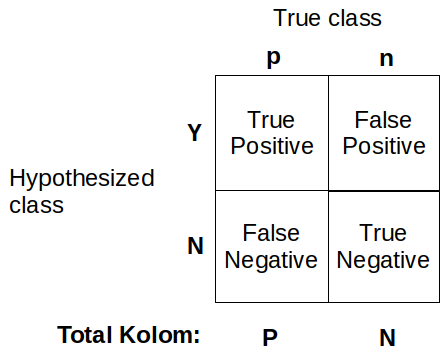
\includegraphics[keepaspectratio=true,scale=0.5]{confusion_matrix}
	\caption{Matriks \textit{confusion}}
	\label{fig:confusion_matrix}
\end{figure}

Laju \textit{true positive} (disebut juga dengan \textit{hit rate} dan
\textit{recall}) dari sebuah pengklasifikasi dapat dihitung dengan,

\begin{align*}
	\textit{tp rate} &\approx
			\frac{\text{Jumlah klasifikasi positif}}
				{\text{Total positif}} \\
		&= \frac{TP}{P}
\end{align*}
Laju \textit{false positive} (disebut juga \textit{false alarm rate}) dari
pengklasifikasi adalah
\begin{align*}
	\textit{fp rate} &\approx \frac{\text{Jumlah klasifikasi negatif}}
			{\text{Total negatif}} \\
		&= \frac{FP}{N}
\end{align*}
Istilah lainnya yang berkaitan dengan kurva ROC adalah,
\[
	\text{precision} = \frac{TP}{TP + FP}
\]
\[
	\text{accuracy} = \frac{TP + TN}{P + N}
\]
\[
	\text{sensitivity} = \text{recall}
\]
\begin{align*}
	\text{specificity}
		&= \frac{\text{Jumlah true negative}}
			{\text{jumlah false positive}
			+ \text{jumlah true negative}} \\
		&= 1 - \textit{fp rate}
\end{align*}
\[
	\text{positive predictive value} = \text{precision}
\]

\subsubsection{Ruang ROC}

Grafik ROC adalah grafik dua dimensi yang mana \textit{tp rate} diplot pada
$ Y $ dan \textit{fp rate} diplot pada sumbu $ X $.
Sebuah grafik ROC menggambarkan lawan antara keuntungan (true positive) dan
biaya (false positive).
Gambar \ref{fig:roc_graph} memperlihatkan grafik ROC dengan lima klasifikasi
dari A sampai E.

\begin{figure}[t!]
	\centering
	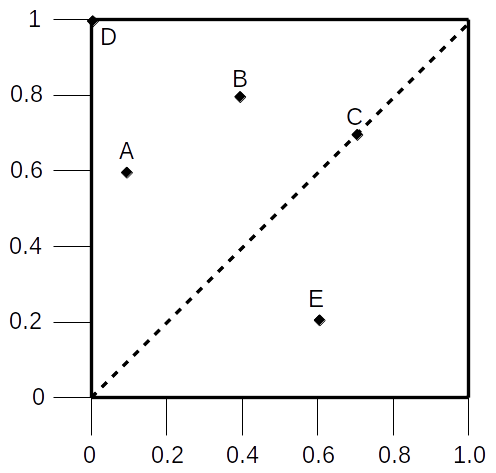
\includegraphics[keepaspectratio=true,scale=0.5]{roc_graph}
	\caption{Grafik ROC dengan lima klasifikasi}
	\label{fig:roc_graph}
\end{figure}

Klasifikasi diskrit yaitu yang mengeluarkan hanya sebuah label kelas.
Setiap pengklasifikasi diskrit menghasilkan sebuah pasangan
(\textit{fp rate}, \textit{tp rate}) yang berkorespondensi dengan satu titik di
ruang ROC.

Titik (0,0) merepresentasikan klasifikasi yang tidak pernah positif dan tidak
pula negatif. Sebaliknya, titik (1,1) merepresentasikan klasifikasi positif.
Titik (0,1) merepresentasikan klasifikasi sempurna, contohnya D.

Titik dalam ruang ROC lebih baik daripada yang lainnya bila berada di bagian
kiri atas (\textit{tp rate} tinggi, \textit{fp rate} rendah, atau keduanya).
Pengklasifikasi yang berada di sisi kiri dari grafik ROC, dekat sumbu $X$, bisa
disebut "konservatif": menghasilkan klasifikasi positif hanya dengan bukti yang
kuat sehingga menghasilkan beberapa galat positif, tapi seringkali memiliki
\textit{tp rate} yang rendah.
Pengklasifikasi di bagian kanan-atas dari grafik ROC bisa disebut "liberal":
menghasilkan klasifikasi positif dengan bukti yang lemah atau menghasilkan
hampir semuanya positif secara tepat, tapi memiliki \textit{fp rate} yang
tinggi.
Pada gambar \ref{fig:roc_graph}, pengklasifikasi $A$ lebih konservatif daripada
$B$.

\subsubsection{Performansi acak}

Garis diagonal $ y = x $ merepresentasikan strategi yang secara acak memilih
kelas.
Sebagai contohnya, jika sebuah pengklasifikasi secara acak memilih kelas
positif, maka didapat setengahnya positif dan setengahnya negatif menghasilkan
titik (0.5,0.5) di ruang ROC.
Jika secara acak mendapatkan 90\% positif, maka \textit{fp rate}-nya juga akan
meningkat menjadi 90\%, menghasilkan titik (0.9,0.9) di ruang ROC.
Pada gambar \ref{fig:roc_graph} klasifikasi C bisa dibilang secara acak menebak
kelas positif 70\%.

Pengklasifikasi yang berada di bawah kanan diagonal bekerja lebih buruk dari
pengklasifikasi yang menerka secara acak.
Bagian ini biasanya kosong dalam grafik ROC.

\subsubsection{Kurva \textit{Area Under ROC}}

Sebuah kurva ROC adalah gambar dua dimensi dari performansi pengklasifikasi.
Untuk membandingkan pengklasifikasi bisa dengan menurunkan performansi ROC
menjadi nilai skalar tunggal merepresentasikan performansi yang diharapkan.
Metode yang paling umum yaitu menghitung wilayah di bawah kurva ROC, disingkat
dengan AUC (\textit{Area Under an ROC}).
Secara AUC adalah bagian dari area dari sebuah bujur sangkar, nilainya akan
selalu antara 0 dan 1.0.
Karena perkiraan secara acak menghasilkan garis diagonal antara (0,0) dan
(1,1), yang memiliki wilayah 0.5, maka tidak ada pengklasifikasi yang 
seharusnya memiliki AUC kurang dari 0.5.

\subsection{Cascaded Random Forests}

Berikut rangkuman dari makalah Baumann dkk. \cite{baumann2013cascaded},

\begin{itemize}
\item Sebuah cascade terdiri dari beberapa \textit{stage} dengan kompleksitas
yang meningkat.
\item Setiap \textit{stage} paling kurang memiliki satu pohon.
\item Pohon ditambahkan ke stage sampai \textit{true positive rate} dan
\textit{true negative rate} dicapai.
\item Label dari sampel ditentukan oleh probabilitas kelas dari \textit{tree}
yang berbeda di stage $S$.
\item Untuk mengurangi pengaruh \textit{stage} yang performansinya rendah maka
ditambahkan faktor bobot $\alpha$ untuk setiap \textit{stage}, yaitu,
\[
	\alpha_{s} = exp(fmeasure)
\]
yang mana $fmeasure$ didapat dari,
\[
	fmeasure = 2 \cdot \frac{precision \cdot recall}{precision + recall}
\]
\item $\alpha_{s}$ secara linear dinormalkan menjadi rentang antara 0 dan 1.
\item Bobot dari \textit{stage} yang memiliki performansi rendah dikurangi
supaya pengaruh mereka pada mayoritas voting berkurang.
\end{itemize}

\begin{algorithm}[t!]
\caption{Algoritma Cascaded Random Forest}
\label{alg:cascadedrf}
\begin{algorithmic}
	\Require \\
	S: jumlah stage \\
	T: maksimum jumlah tree di setiap stage \\
	mintp: ambang batas untuk nilai minimum true positive \\
	mintn: ambang batas untuk nilai minimum true negative \\
	\Function{CascadedRandomForest}{$S, T, mintp, mintn$}
		\For{$ s = 1 \to S $}
			\For{$ t = 1 \to T $}
				\State buat \textit{tree}
				\If{$TP_{s,t} > mintp $ AND $ TN_{s,t} > mintn $}
					\State stage selesai.
				\EndIf
			\EndFor
			\State Hitung bobot $ \alpha = exp(fmeasure) $
			\State Hapus \textit{true-negative}
			\State Isi ulang dengan \textit{false-positive}
		\EndFor
	\EndFunction
\end{algorithmic}
\end{algorithm}

Dari algoritma Cascaded Random Forest \ref{alg:cascadedrf}, ada beberapa
pertanyaan untuk makalah tersebut,
\begin{itemize}
\item Untuk jenis dataset multi-kelas bukankah nilai TN sama dengan TP? Yang
mana TN = 1 - FP Rate.
\item Apa yang harus dilakukan jika maksimum jumlah tree tercapai tapi nilai
$TP_{s,t}$ dan $TN_{s,t}$ tidak mencapai $mintp$ dan $mintn$?
\item Apa yang dimaksud dengan "Hapus \textit{true negative}"? Apakah dihapus
stagenya? Treenya? Samplenya? Makalah tidak secara eksplisit menjelaskan
bagian ini
\item Apa yang dimaksud dengan "Isi ulang dengan \textit{false-positive}"?
\end{itemize}

Karena masih ada yang belum dipahami pada algoritmanya, implementasi
\textit{Cascaded Random Forest} untuk pengklasifikasi dataset multi-kelas belum
selesai.


\clearpage
\section{Pekerjaan Selanjutnya}

Berikut garis besar tahap yang akan dikerjakan untuk pekerjaan selanjutnya,

\begin{itemize}
\item perbaikan implementasi \textit{Cascaded Random Forest}.
\item Implementasi algoritma LN-SMOTE.
\item Implementasi fitur vandalisme di Wikipedia.
\item Menerapkan algoritma SMOTE dan LN-SMOTE pada hasil penghitungan fitur.
\item Menerapkan \textit{Random Forest} pada hasil \textit{resampling} SMOTE
dan LN-SMOTE.
\item Menerapkan algoritma \textit{Cascade Random Forest} dari hasil SMOTE dan
LN-SMOTE.
\item Analisis hasil dari klasifikasi \textit{Random Forest} dan
\textit{Cascaded Random Forest}.
\end{itemize}

\clearpage
\schedule{4}{14}{0}{0}

\advisorsignature

\clearpage
\addcontentsline{toc}{section}{Daftar Referensi}
\printbibliography

\newpage
\appendix
\begin{itemize}
\item \textbf{Minggu 15, 16}. Perbaikan program CART dan implementasi Random
Forest.
\end{itemize}


\end{document}
